% atifcppprogrammers's Data Communication Lab Report #5%
\documentclass[fullpage]{article}
\usepackage{tgpagella}
\usepackage{graphicx}
\usepackage{float}
\usepackage[english]{babel}
\usepackage[latin1]{inputenc}

\begin{document}

   \title{Experiment 5 - Building Topologies in NS3}

   \author{Muhammad Atif Farooq L144392 EE}

   \date{3rd October 2019}

   \maketitle

\section{Introduction}
Having implemented the point to point, CSMA and Wi-Fi topologies, it is then natural
to extend our investigation to the  star topology network. For the star topology a predefined
number of nodes are connected to a central Hub (packet sink), in a manner
similar to the spokes on a wheel.

The intent being that once these nodes are properly configured and equipped
with the right application,s they will send packets to the sink in a sequential manner,
and then await acknowledgment.

\section{Objective}
Implement and analyze the star topolgy in NS3.

\section{Procedure}
For the lab task we were instructed to first study the \verb|examples/tcp/star.cc| script
and which was intended to implement a standard star topology with $n=8$ spoke nodes
and a central Hub, consequently the topology was constituted by $n+1 = 9$ nodes
in total, as presented in the figure below.

\begin{figure}[H]
  
\includegraphics[width=\linewidth]{starTopology.png}
  \caption{starTopology.png}
  \label{fig:output0}
\end{figure}

Having studied the code required to model the standard star topolgy, we were then
required to write code to model a slightly different topology, the details are discussed in
the section below.

\subsection{The Topology}
In contrast to the topology presented in \verb|examples/tcp/star.cc|, the lab task
instructed us to install the packet sink application on node nine, in addition we
were to refrain from installing any applications on nodes zero and five. An illustration
of the required topology is discussed below.

\begin{figure}[H]
  
\includegraphics[width=\linewidth]{labQuestionTopology.png}
  \caption{labQuestionTopology.png}
  \label{fig:output1}
\end{figure}

\subsection{Stratedgy Employed}
To implement the topology in question, we first created the standard star topology and then
a point to point link between nodes five and nine, installing the net devices and protocol
stacks required by all the nodes for both the start and p2p link.

After assigning IPs, to ensure the packet sink application was installed on node nine we used
the corresponding IP address stored in the interfaces for the p2p nodes. The remaining key
ideas can be inferred from the code and console output presented below.

\subsection{Code and Console Output}

\begin{verbatim}
  #include "ns3/core-module.h"
  #include "ns3/network-module.h"
  #include "ns3/netanim-module.h"
  #include "ns3/internet-module.h"
  #include "ns3/point-to-point-module.h"
  #include "ns3/applications-module.h"
  #include "ns3/point-to-point-layout-module.h"

  using namespace ns3;

  NS_LOG_COMPONENT_DEFINE ("Star");

  int
  main (int argc, char *argv[])
  {

    // Adding Log Levels for Console Output.
    LogComponentEnable("Star",LOG_LEVEL_INFO);
    LogComponentEnable("PacketSink",LOG_LEVEL_INFO);
    LogComponentEnable("OnOffApplication",LOG_LEVEL_INFO);
    NS_LOG_INFO("Star Topolgy Simulation");

    //
    // Set up some default values for the simulation.
    //
    Config::SetDefault ("ns3::OnOffApplication::PacketSize", UintegerValue (137));

    // ??? try and stick 15kb/s into the data rate
    Config::SetDefault ("ns3::OnOffApplication::DataRate", StringValue ("14kb/s"));

    //
    // Default number of nodes in the star.  Overridable by command line argument.
    //
    uint32_t nSpokes = 8;

    CommandLine cmd;
    cmd.AddValue ("nSpokes", "Number of nodes to place in the star", nSpokes);
    cmd.Parse (argc, argv);

    // Specifying attributes for point tp point links of star topology.
    NS_LOG_INFO("Building Star Topology.");
    PointToPointHelper pointToPoint;
    pointToPoint.SetDeviceAttribute ("DataRate", StringValue ("5Mbps"));
    pointToPoint.SetChannelAttribute ("Delay", StringValue ("2ms"));
    PointToPointStarHelper star (nSpokes, pointToPoint);

    // Installing internet stack on all nodes of start topology.
    NS_LOG_INFO("Installing internet stack on nodes of star topology");
    InternetStackHelper internet;
    star.InstallStack (internet);

    // Assigning IP Address to nodes of star topology.
    NS_LOG_INFO ("Assign IP Addresses.");
    star.AssignIpv4Addresses (Ipv4AddressHelper ("10.1.1.0", "255.255.255.0"));

    // Creating point to point link for connection between node 5 and node 9.
    NodeContainer p2pNodes;
    p2pNodes.Add(star.GetSpokeNode(4));
    p2pNodes.Create(1);

    // Installing netdevices, internet stack and assigning ip's for this link.
    NetDeviceContainer p2pDevices;
    p2pDevices = pointToPoint.Install(p2pNodes);

    internet.Install(p2pNodes.Get(1));

    Ipv4AddressHelper address;
    address.SetBase ("10.2.1.0", "255.255.255.0");

    Ipv4InterfaceContainer interfaces = address.Assign (p2pDevices);

    // Installing Hub App on Node 9, (making it the packet sink).
    uint16_t port = 50000;
    Address hubLocalAddress (InetSocketAddress (Ipv4Address::GetAny (), port));
    PacketSinkHelper packetSinkHelper ("ns3::TcpSocketFactory", hubLocalAddress);
    ApplicationContainer hubApp = packetSinkHelper.Install (p2pNodes.Get(1));
    hubApp.Start (Seconds (1.0));
    hubApp.Stop (Seconds (10.0));

    // Installing on off applications.
    OnOffHelper onOffHelper ("ns3::TcpSocketFactory", Address ());
    onOffHelper.SetAttribute ("OnTime",
      StringValue ("ns3::ConstantRandomVariable[Constant=1]"));
    onOffHelper.SetAttribute ("OffTime",
      StringValue ("ns3::ConstantRandomVariable[Constant=0]"));

    ApplicationContainer spokeApps;

    for (uint32_t i = 0; i < star.SpokeCount (); ++i)
      {
        if(i == 0 || i == 4) continue;
        AddressValue remoteAddress (InetSocketAddress
          (interfaces.GetAddress(1), port));
        onOffHelper.SetAttribute ("Remote", remoteAddress);
        spokeApps.Add (onOffHelper.Install (star.GetSpokeNode (i)));
      }
    spokeApps.Start (Seconds (1.0));
    spokeApps.Stop (Seconds (10.0));

    NS_LOG_INFO ("Enable static global routing.");
    //
    // Turn on global static routing so we can actually be routed across the star.
    //
    Ipv4GlobalRoutingHelper::PopulateRoutingTables ();

    NS_LOG_INFO ("Enable pcap tracing.");
    //
    // Do pcap tracing on all point-to-point devices on all nodes.
    //
    pointToPoint.EnablePcapAll ("atif_star");

    NS_LOG_INFO ("Run Simulation.");
    Simulator::Run ();
    Simulator::Destroy ();
    NS_LOG_INFO ("Done.");

    return 0;
  }
\end{verbatim}

\begin{figure}[H]
  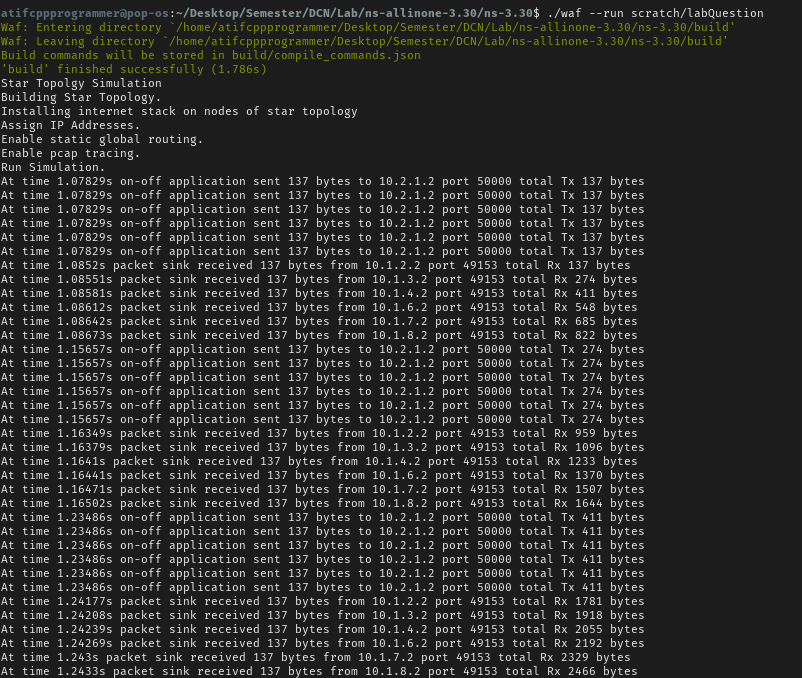
\includegraphics[width=\linewidth]{labQuestion.png}
  \caption{labQuestion.cc}
  \label{fig:output2}
\end{figure}

\section{Conclusions}
NS3 can be used to model an analyze star topologies.

\section{Post-Lab Question}
For the post lab we were required to implement the following topology, the code
and console output are presented below.

\begin{figure}[H]
  
\includegraphics[width=\linewidth]{postLabQuestionTopology.png}
  \caption{postLabQuestionTopology.png}
  \label{fig:output3}
\end{figure}

\begin{verbatim}
  #include "ns3/core-module.h"
  #include "ns3/csma-module.h"
  #include "ns3/network-module.h"
  #include "ns3/netanim-module.h"
  #include "ns3/internet-module.h"
  #include "ns3/point-to-point-module.h"
  #include "ns3/applications-module.h"
  #include "ns3/ipv4-global-routing-helper.h"
  #include "ns3/point-to-point-layout-module.h"

  using namespace ns3;

  NS_LOG_COMPONENT_DEFINE ("Star");

  int
  main (int argc, char *argv[])
  {
    // Enabling log components for console output.
    LogComponentEnable("Star",LOG_LEVEL_INFO);
    LogComponentEnable("PacketSink",LOG_LEVEL_INFO);
    LogComponentEnable("OnOffApplication",LOG_LEVEL_INFO);

    // Check to see if loging is enabled.
    NS_LOG_INFO("atifcppprogrammer's post_lab_question");

    // Setting up default values for the simulation.
    Config::SetDefault ("ns3::OnOffApplication::PacketSize", UintegerValue (137));
    Config::SetDefault ("ns3::OnOffApplication::DataRate", StringValue ("14kb/s"));

    // Defining spoke count for star and node count for csma.
    uint32_t nSpokes = 8,nCsma = 4;

    // Case user wishes to ammend above spoke and csma counts at the outset.
    CommandLine cmd;
    cmd.AddValue ("nSpokes", "Number of nodes to place in star", nSpokes);
    cmd.AddValue ("nCsma", "Number of nodes to place in csma", nCsma);
    cmd.Parse (argc, argv);

    // Building our star topology.
    NS_LOG_INFO(" 1. Building our star topology");
    PointToPointHelper pointToPoint;
    pointToPoint.SetDeviceAttribute("DataRate",StringValue("5Mbps"));
    pointToPoint.SetChannelAttribute("Delay",StringValue("2ms"));
    PointToPointStarHelper star (nSpokes,pointToPoint);

    // Creating nodes for csma channel.
    NS_LOG_INFO(" 2. Creating nodes for csma channel");
    NodeContainer csmaNodes;
    csmaNodes.Create(nCsma);

    // Defining attributes of csma channel.
    NS_LOG_INFO(" 3. Defining attributes of csma channel");
    CsmaHelper csma;
    csma.SetChannelAttribute ("DataRate", StringValue ("100Mbps"));
    csma.SetChannelAttribute ("Delay", TimeValue (NanoSeconds (6560)));

    // Installing network cards on csma channel.
    NS_LOG_INFO(" 4. Installing network cards for csma nodes");
    NetDeviceContainer csmaDevices;
    csmaDevices = csma.Install(csmaNodes);

    // Installing internet stack on star and csma nodes.
    NS_LOG_INFO(" 5. Installing protocol stack on star and csma nodes");
    InternetStackHelper stack;
    stack.Install(csmaNodes); star.InstallStack(stack);

    // Creating node container for nodes 5 and 9.
    NS_LOG_INFO(" 6. Create node container for node 5 of star and node 9 of csma");
    NodeContainer p2pNodes = NodeContainer(star.GetSpokeNode(4),csmaNodes.Get(0));

    // Installing Network Cards for p2p nodes.
    NS_LOG_INFO(" 7. Installing additional network cards on p2p nodes");
    NetDeviceContainer p2pDevices;
    p2pDevices = pointToPoint.Install(p2pNodes);

    // Assigning IP Addresses for star topology.
    NS_LOG_INFO("10. Assigning IP Address for star nodes");
    star.AssignIpv4Addresses (Ipv4AddressHelper ("10.1.1.0", "255.255.255.0"));

    // Assigning IP Addresses  for p2p nodes.
    NS_LOG_INFO("11. Assigning IP Address for p2p nodes");
    Ipv4AddressHelper address;
    address.SetBase ("10.2.1.0", "255.255.255.0");
    Ipv4InterfaceContainer p2pInterfaces;
    p2pInterfaces = address.Assign (p2pDevices);

    // Assigning IP Addresses  for csma nodes.
    address.SetBase ("10.3.1.0", "255.255.255.0");
    Ipv4InterfaceContainer csmaInterfaces;
    csmaInterfaces = address.Assign (csmaDevices);

    // Creating Applications.
    NS_LOG_INFO("12. Creating OnOff and Hub Applications");

    // Creating a packet sink on node 12 of csma channel.
    uint16_t port = 50000;
    Address hubLocalAddress (InetSocketAddress (Ipv4Address::GetAny (), port));
    PacketSinkHelper packetSinkHelper ("ns3::TcpSocketFactory", hubLocalAddress);
    ApplicationContainer hubApp = packetSinkHelper.Install (csmaNodes.Get(nCsma-1));
    hubApp.Start (Seconds (1.0));
    hubApp.Stop (Seconds (10.0));

    // Creating OnOff apps to send tcp packets to hub, on on each spoke node.
    OnOffHelper onOffHelper ("ns3::TcpSocketFactory", Address ());
    onOffHelper.SetAttribute ("OnTime",
      StringValue ("ns3::ConstantRandomVariable[Constant=1]"));
    onOffHelper.SetAttribute ("OffTime",
      StringValue ("ns3::ConstantRandomVariable[Constant=0]"));

    ApplicationContainer spokeApps;

    for (uint32_t i = 0; i < star.SpokeCount (); ++i){
      // Skipping installation of apps on node 0 and node 4.
      if (!(i == 0 || i == 4)){
        AddressValue remoteAddress (InetSocketAddress
          (csmaInterfaces.GetAddress(nCsma-1), port));
        onOffHelper.SetAttribute ("Remote", remoteAddress);
        spokeApps.Add (onOffHelper.Install (star.GetSpokeNode (i)));
      }
    }
    spokeApps.Start (Seconds (1.0));
    spokeApps.Stop (Seconds (10.0));

    // Enabling global routing.
    NS_LOG_INFO ("13. Enabling static global routing");
    Ipv4GlobalRoutingHelper::PopulateRoutingTables();

    // Running program.
    NS_LOG_INFO ("14. Running Simulation");
    Simulator::Run ();
    Simulator::Destroy ();

    // Ok ! we are done now.
    NS_LOG_INFO ("Done !!!");

    return 0;
  }
\end{verbatim}

\begin{figure}[H]
  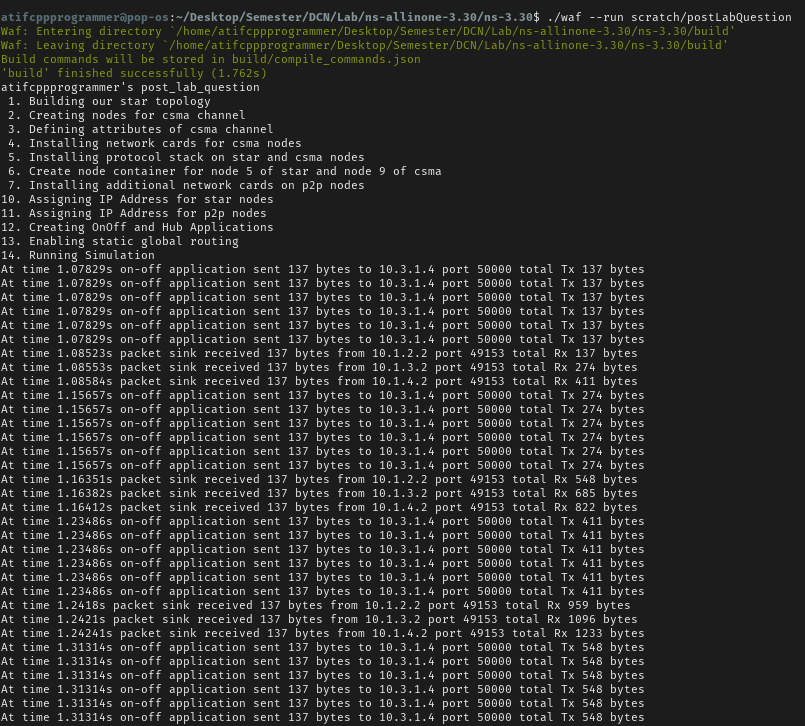
\includegraphics[width=\linewidth]{postLabQuestion.png}
  \caption{postLabQuestion.cc}
  \label{fig:output4}
\end{figure}

\end{document}
